\chapter{功能仿真结果}

\section{利用Chisel3配套工具进行快速仿真}
Chisel3在Github网站上有一套基于Scala体系的仿真工具,chisel-testers。
使用该工具可以直接在Scala中实例化使用Chisel3开发的模块,并且产生激励进行模块的仿真。
其主要提供了一个名为PeekPokeTester的类,该类提供了能够完成激励产生和信号断言的方法。
\begin{table}[h] %开始一个表格environment,表格的位置是h,here。  
    \centering
    \caption{PeekPokeTester中提供的方法} %显示表格的标题  
    \begin{tabular}{l|l|c} %设置了每一列的宽度,强制转换。  
    \hline  
    \hline  
    方法名 & 作用 & 使用举例 \\ %用&来分隔单元格的内容 \\表示进入下一行  
    \hline %画一个横线,下面的就都是一样了,这里一共有4行内容  
    poke & 设置DUT的输入信号 & poke(c.io.in.valid, 1) \\
    \hline  
    peek & 读取DUT的输出信号 & peek(c.io.out.bits) \\
    \hline  
    expect & 比较DUT的输出信号 & expect(c.io.out.bit, 0xff) \\
    \hline  
    step & 驱动DUT的时钟信号 & step(1) \\
    \hline
    reset & 驱动DUT的复位信号 & reset(1) \\
    \hline  
    \hline  
    \end{tabular}  
\end{table}
同时,该工具支持使用Verilator作为仿真后端,大大降低了大规模电路的仿真时间,借助Verilator,可以产生仿真时的vcd仿真文件,通过GTKWave、Verdi等波形查看工具即可查看仿真波形,
使用时十分便利。相比于Verilog环境下编写行为复杂的testbench,Chisel-Tester提供的解决方案依赖于面向对象编程,逻辑更加清晰,不易出错。
            \begin{lstlisting}[title=Chisel Test Example, frame=shadowbox]
class Tester(c: Test) extends PeekPokeTester(c) {
  poke(c.io.in, -1)     //Set DUT input "in" as -1
  step(1)               //wait 1 clock
  expect(c.io.out, -1)  //assert DUT output "out" as -1
}
            \end{lstlisting}

\section{基于FIFO的可变长移位寄存器仿真结果}
% filters: DenseVector(0, 2, -1) __ 3
% filterNum: 1
% imgs: DenseVector(4, -3, -3, -1, -5) __ 5
% imgNum: 1
% nchannel: 1
\begin{figure}[h]
    \centering
    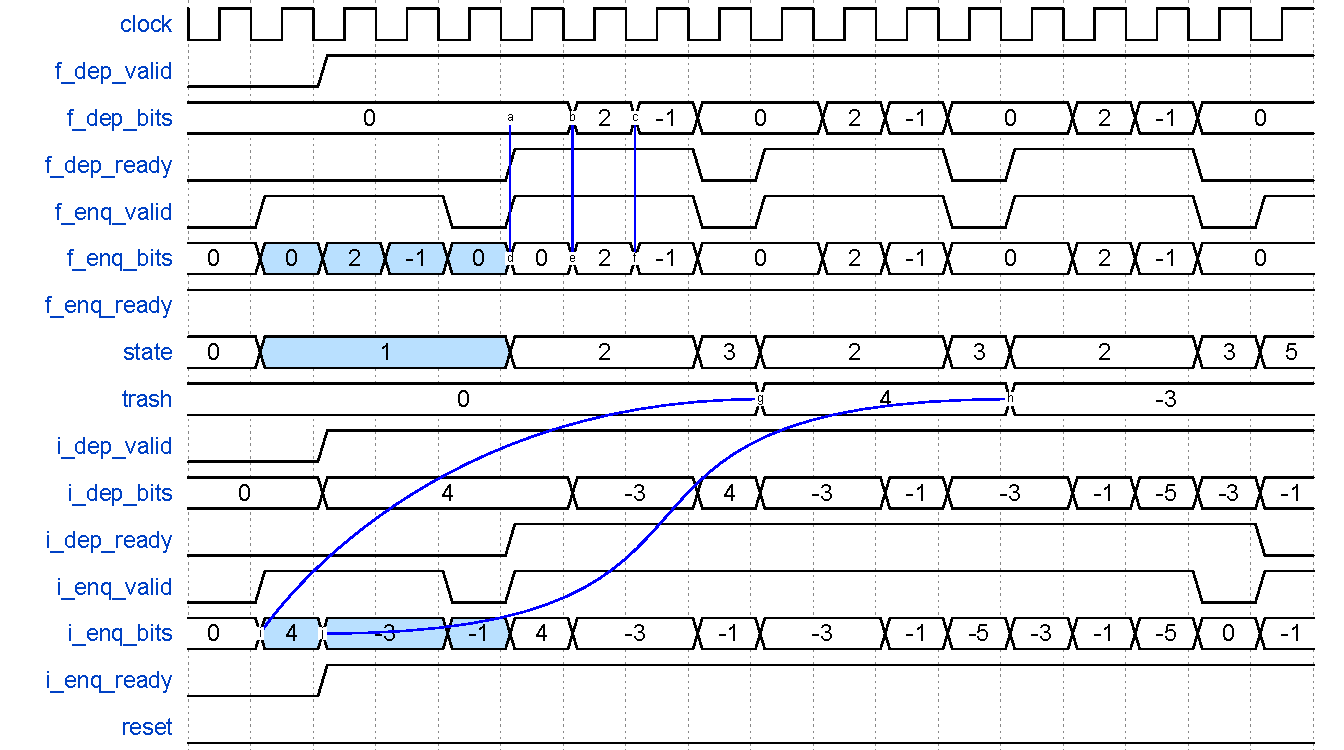
\includegraphics[scale=0.7]{../pdf/shift_w.pdf}\\
    \caption{基于FIFO的可变长移位寄存器仿真波形图}
    \label{shift_w}
\end{figure}
该模块的逻辑行为切换由\emph{state}信号控制。
当\emph{state=0}时该模块不工作,
\emph{state=1}时,模块内嵌的FIFO输入接口通过Mux与外部输入数据接口对接,此时开始存储外部数据,如图\ref{shift_w}阴影部分所示,此时filter FIFO中依次存入了0,-2,-1,img FIFO中依次存入了4,-3,-3。
\emph{state=2}时,模块内嵌FIFO输入接口通过Mux与自身的输出接口对接,形成环路,此时被弹出的数据再次回到FIFO中以完成循环移位寄存器的功能,如图\ref{shift_w},\emph{f\_dep}信号组中出现的连接线,弹出的0,2,-1同时又写回FIFO。
\emph{state=3}时,模块中FIFO数据已经全部计算完成,根据卷积计算的特性,此时需要弹出部分数据之后接受等长的新数据,由于FIFO输入接口与输出接口互不干扰,因此可以弹出废弃数据的同时接受新的数据,如图\ref{shift_w}\emph{i\_enq}和\emph{i\_deq}信号组中的连接线,最开始存入的4,-3分别在两次中弹出,同时两次中分别接受了-1,-5两个新数据。
% \begin{figure}[h]
%     \centering
%     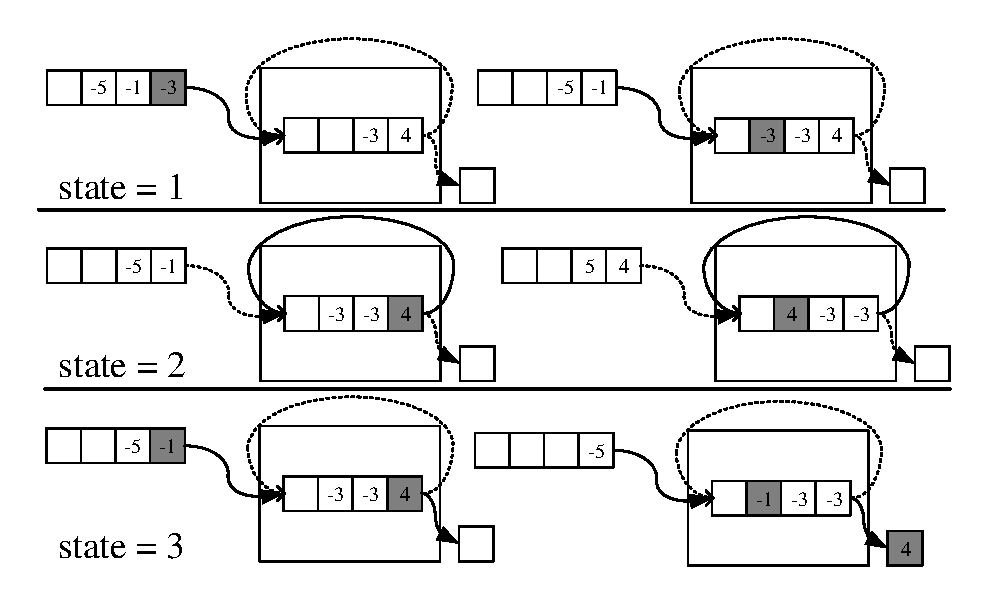
\includegraphics[scale=0.8]{../pdf/shift_k.pdf}\\
%     \caption{基于FIFO的可变长移位寄存器工作示意图}
%     \label{shift_k}
% \end{figure}
该模块的工作示意图可以参考\ref{shift_k}。

\section{Designware SRAM IP仿真结果}
\begin{figure}[h]
    \centering
    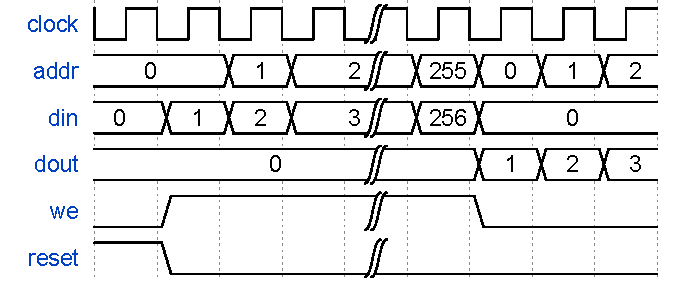
\includegraphics{../pdf/sram_w.pdf}\\
    \caption{SRAM IP波形图}
    \label{sram_w}
\end{figure}
仿真时序图\ref{sram_w}前半段写信号\emph{we}为高,依次向256个\emph{addr}写入值为\emph{addr+1}的数据,
后半段\emph{we}为低,开始读数据,依次从256个\emph{addr}中读出值为\emph{addr+1}的数据。
从时序图可以判断,该SRAM IP读取阶段为异步方式,输出信号\emph{dout}与时钟上升沿无关,直接与输入地址\emph{addr}有关。
这符合本文PE中对SRAM异步读取的需求。

\section{PE单元仿真结果}
时序图\ref{pe_w}显示的是单通道、单卷积核、单图片的$[4,-3,-3,-1,-5] * [0,2,-1]$的完整计算过程。
\begin{figure}[h]
    \centering
    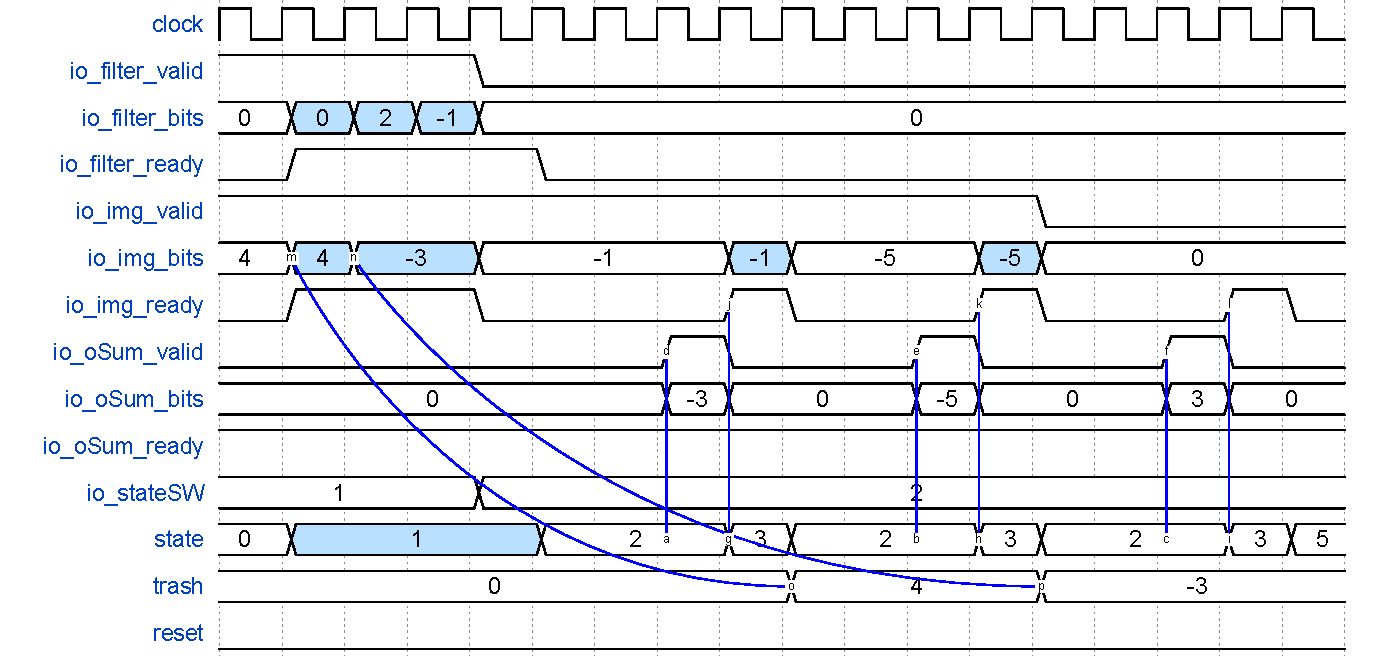
\includegraphics[scale=0.7]{../pdf/pe_w.pdf}\\
    \caption{PE波形图}
    \label{pe_w}
\end{figure}
当\emph{state=1}时,PE内部的img FIFO和filter FIFO开始存数,图\ref{pe_w}阴影背景的数据为存入FIFO的数据,filter FIFO依次存入$0,2,-1$,
img FIFO首先一次性存入$4,-3,-3$,然后当\emph{state=3}时,读入$-1$和$-5$,同时依次弹出$4$和$-3$,FIFO内数据总长度保持不变,如图\ref{pe_w}左侧两条曲线所示。
当\emph{state=2}时,PE开始进行计算此阶段末期会将计算结果通过\emph{oSum}信号弹出,弹出数据个数等于$fNum*iNum$,此过程重复数次,直至外部img FIFO为空时,计算结束\emph{state=5}


\section{PE阵列仿真结果}
\begin{figure}[h]
    \centering
    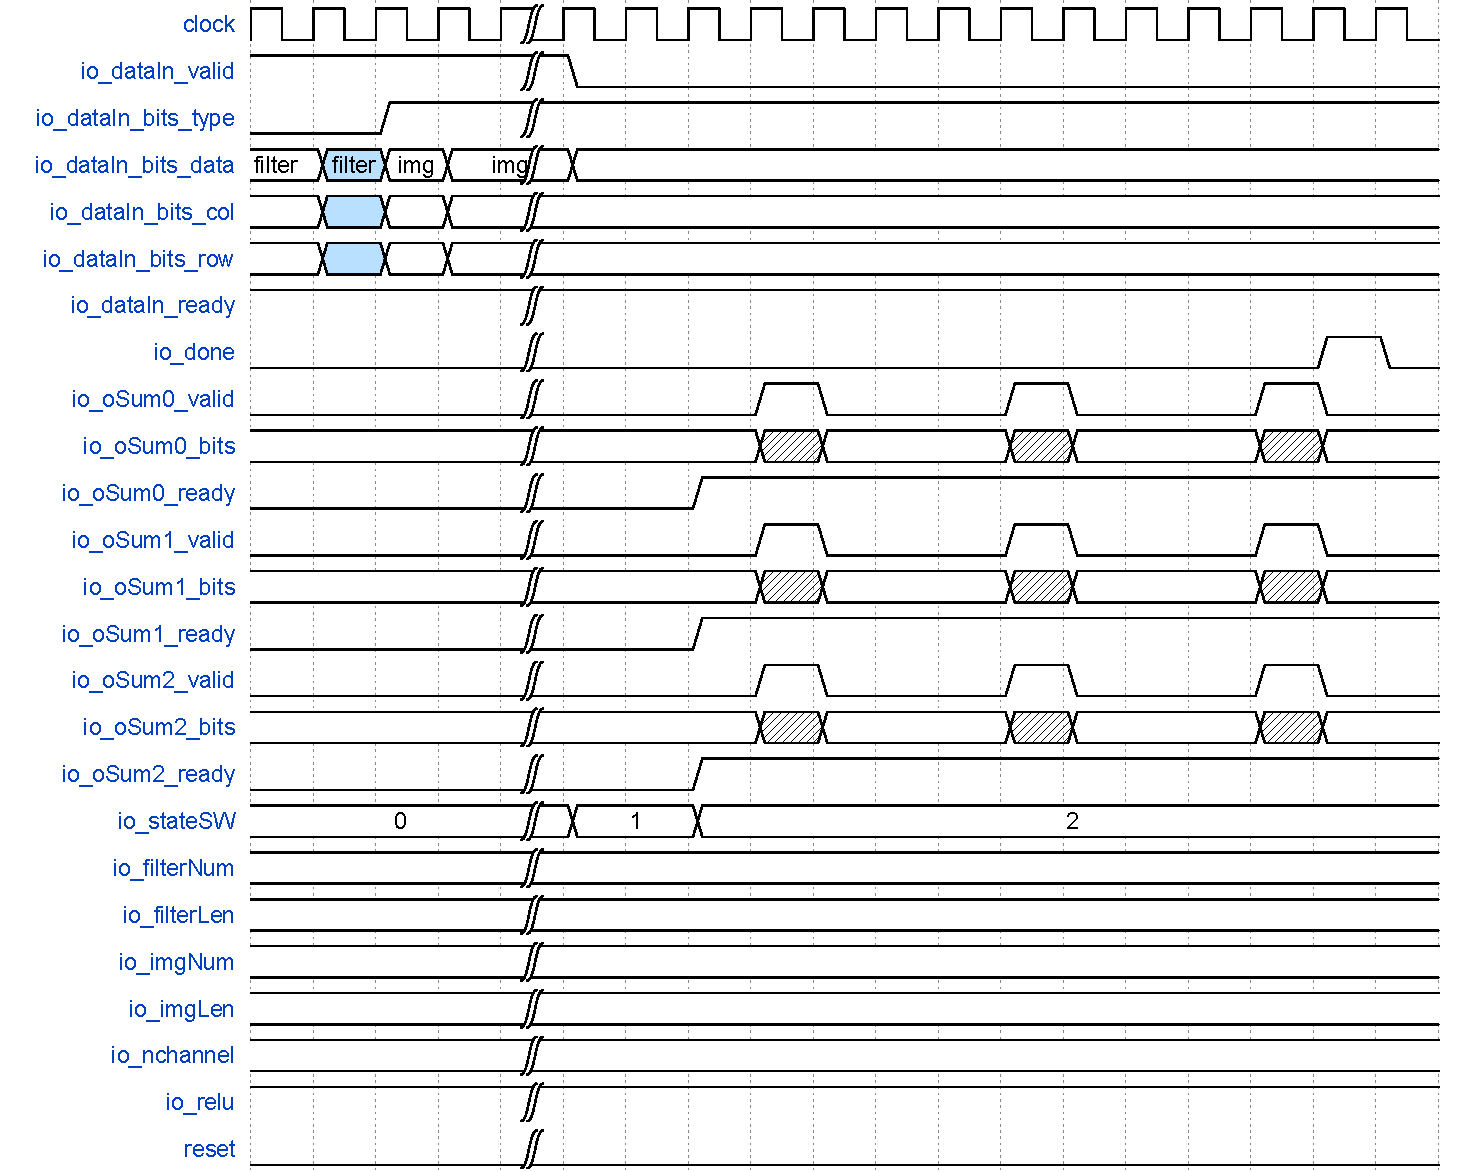
\includegraphics[scale=0.65]{../pdf/pearray_w.pdf}\\
    \caption{PEArray波形图}
    \label{pearray_w}
\end{figure}
PE阵列的计算可以等效为多个PE计算单元计算结果的叠加,其输出通道数\emph{oSumX}等于PE阵列的列数,输出的数据为每列PE输出数据递归加。
由于所有PE单元都处在相同的始终域,且输入的数据长度必定相等,因此他们的计算必定会同步完成。

时序图\ref{pearray_w}展现了一个完成的PE阵列计算过程的示意图,
第一阶段\emph{state=0}数据从模块端口输入,存入PE外部FIFO中,其完整输入数据包括数据类型、数据地址、实际数据,NoC网络通过判断地址决定是否允许数据通过进入PE外部FIFO中,
同时,PE根据数据类型判断数据时img还是filter。

然后当\emph{state=1}时,数据从PE外部FIFO进入PE内部FIFO,当\emph{state=2}时PE阵列开始进行计算工作,直至外部img FIFO为空,此时done信号置1,
代表所有数据均计算完毕,done信号可以作为CPU的中断信号。

下一轮计算对整个阵列进行一次复位,重复上述过程即可。
% [info] [0.405] filterNum: 3
% [info] [0.405] imgNum: 2
% [info] [0.405] channel: 3
% [info] [0.405] fLen: 3
% [info] [0.405] iLen: 5
% [info] [0.405] List(-3, -4, -3, -5, -3, 2, 1, -1, -4, -2, 2, -1, -1, 0, -2, -1, -4, -5, 4, -1, -4, -3, -5, -5, 1, 4, -3)
% [info] [0.405] 
% [info] [0.405] List(4, 0, 3, -4, 3, 4, -3, 2, 0, 4, 1, 0, -1, 1, 4, 0, 0, -3, 1, 1, -5, 1, 2, -5, -3, -4, -3)
% [info] [0.405] 
% [info] [0.405] List(3, 4, -4, 1, 1, 4, -3, -1, 1, 1, -4, -3, -4, -2, -3, 4, -4, -3, 3, -4, -4, 1, -2, 3, -4, 4, 1)
% [info] [0.405] 
% [info] [0.405] img2d: 
% [info] [0.406] List(3, 0, -4, -5, -2, 1, 2, 2, -2, 0, 2, -1, -4, 0, 2, -1, 2, 0, 2, -4, -1, 1, -4, 2, -3, 4, 2, 3, 1, 0)
% [info] [0.406] 
% [info] [0.406] List(-5, -5, 4, 1, -4, -2, 0, 4, -2, -3, 0, -2, 0, -2, 2, -2, 3, 0, 2, 0, 1, 1, -5, -2, 4, -4, 0, -2, -4, -5)
% [info] [0.406] 
% [info] [0.406] List(-1, 0, -4, -2, 2, 3, 0, 4, 2, -1, 4, -5, 0, 3, -1, 0, 0, 0, 4, 2, 2, -4, -2, -5, 2, 3, -4, 1, 3, 2)
% [info] [0.406] 
% [info] [0.406] List(2, 2, 1, 2, -1, 0, -4, -3, -5, 3, -3, 1, 4, 0, 2, -5, 1, -2, 0, -2, 1, 2, 0, -3, -1, 1, 2, 4, 2, -2)
% [info] [0.406] 
% [info] [0.406] List(4, -5, 2, 3, 1, -4, -1, -5, 4, 1, 4, 0, -3, -4, -2, -4, 1, -2, -2, 0, 4, 0, 3, -4, 1, -5, 4, 4, -3, -4)
% [info] [0.406] 
% [info] [0.406] sw: 
% [info] [0.407] 11  40  0  
% 46  0   0  
% 0   32  0  
% [info] [0.407] 
% [info] [0.408] 0   0    5  
% 10  103  7  
% 40  0    0  
% [info] [0.408] 
% [info] [0.408] 0  46  75  
% 0  33  50  
% 0  0   0   
% [info] [0.408] 
% [info] [0.408] 12  22  60   
% 48  8   65   
% 0   0   112  
% [info] [0.408] 
% [info] [0.408] 15  10  0   
% 0   56  0   
% 0   0   20  
% [info] [0.408] 
% [info] [0.408] 38  0   0  
% 93  32  0  
% 17  1   0  
% [info] [0.408] 
% [info] [0.576] jj reduce: 54
% [info] [0.576] sw1d: 54
% [info] [0.583] loop: 1
% [info] [0.583] ===============ERROR: 0======================


\section{运行MNIST测试结果}
    \subsection{模型量化}
    传统神经网络中大多采用浮点数进行训练,因为浮点数精度高,利于反向传播的计算,加快模型收敛,因此推断过程一般也直接采用训练好的浮点数模型进行计算。
    但随着神经网络技术和小型嵌入式设备的发展,人们慢慢发现利用浮点数进行推断的计算代价太高,因此涌现出一些模型量化方法,通过使用定点数来代替浮点数进行运算,在最大限度保持精度的同时,减少计算量。
    例如Google的TensorflowLite,腾讯的ncnn,阿里巴巴的MNN,都是轻量级的深度神经网络推理引擎,针对手机设备进行优化,目前已经大量应用于APP中。

    本文所使用的Int8量化LeNet模型数据来自于https://github.com/jneless/EyerissF。

    \subsection{运行流程}
\begin{figure}[h]
    \centering
    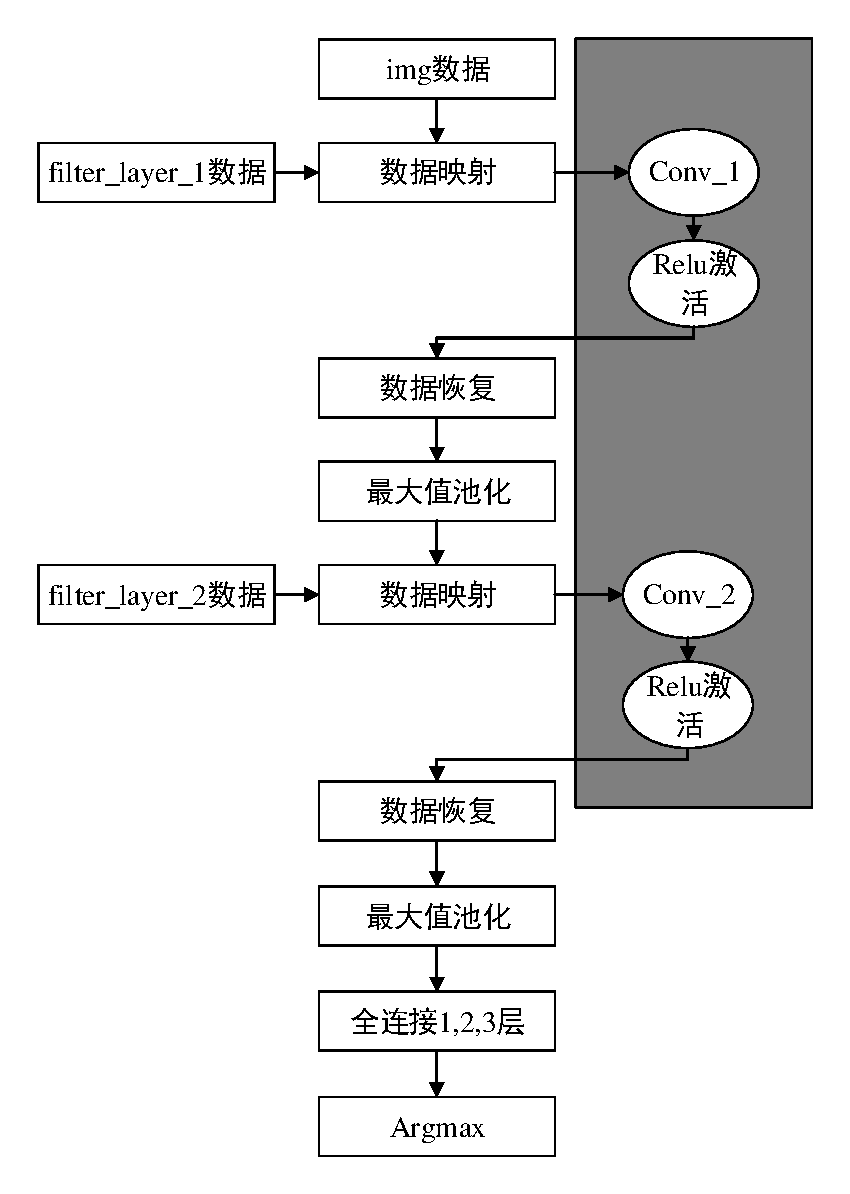
\includegraphics[scale=0.7]{../pdf/MNIST.pdf}\\
    \caption{MNIST仿真流程}
    \label{mnist_k}
\end{figure}
    运行MNIST LeNet测试的流程可以参考图\ref{mnist_k},测试的PE阵列为5×7,图中阴影背景部分为硬件加速器处理过程。
    本文所设计的加速器旨在为卷积层进行加速,以缩短占用全部时长85\%的卷积计算。
    测试时,由软件实现读取存入文本的filter、img数据,并将数据按照图\ref{pe_data}进行组合,图中数据映射主要工作为将图片数据进行切割,以满足5×7阵列一次最大只能接受11($5 + 7 - 1$)行图片数据的限制。
    数据恢复的工作为,将因数据映射分批次计算出来的结果进行连接,组成完整的卷积结果。
    通过该流程即可从行为级层次判断本文设计的卷积加速器能否正常工作。
    \subsection{测试结果}
\begin{figure}[h]
    \centering
    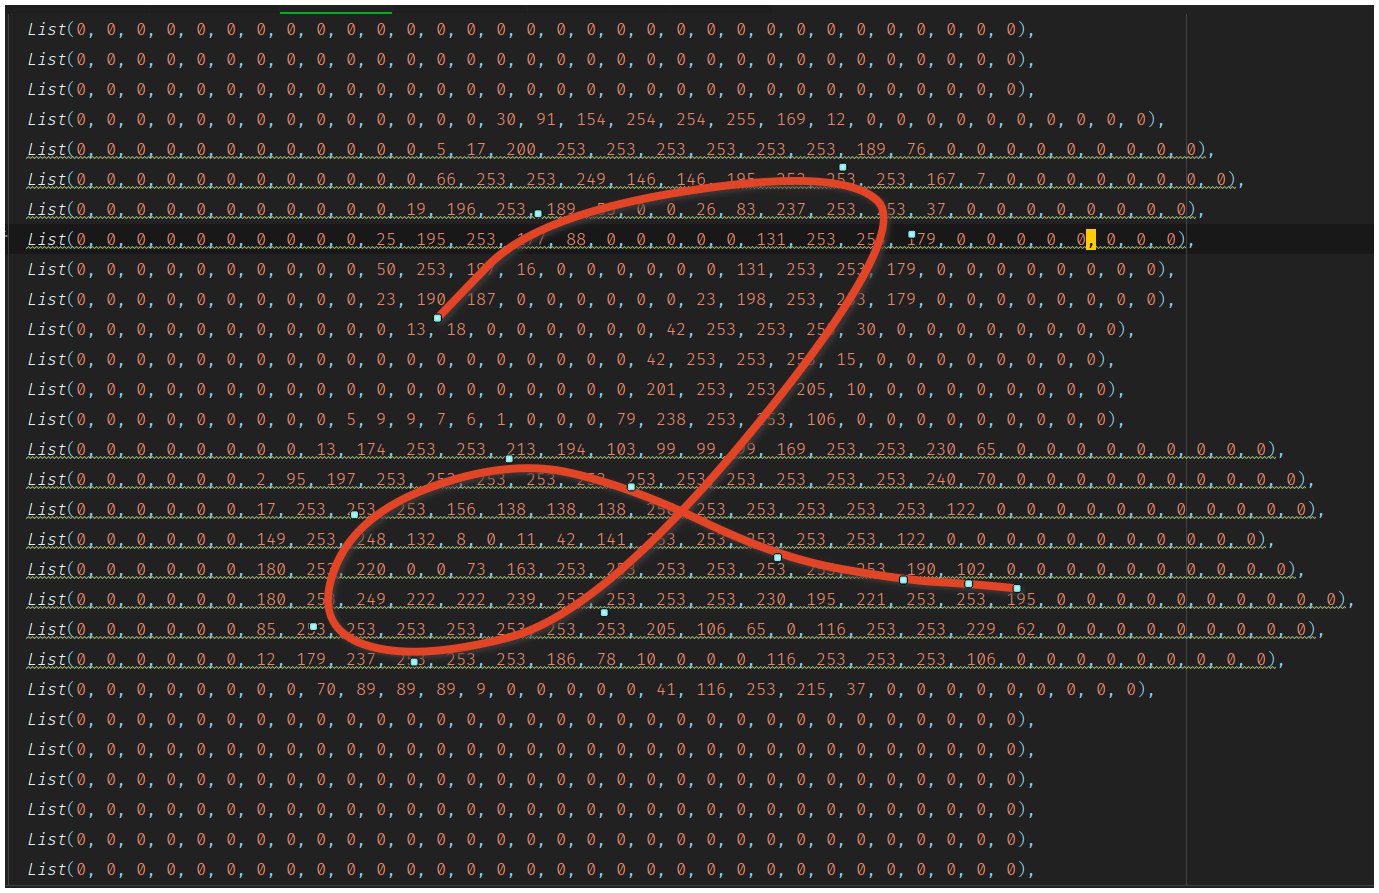
\includegraphics[scale=0.3]{../pdf/2.png}\\
    \caption{输入数据2}
    \label{2}
\end{figure}
\begin{figure}[h]
    \centering
    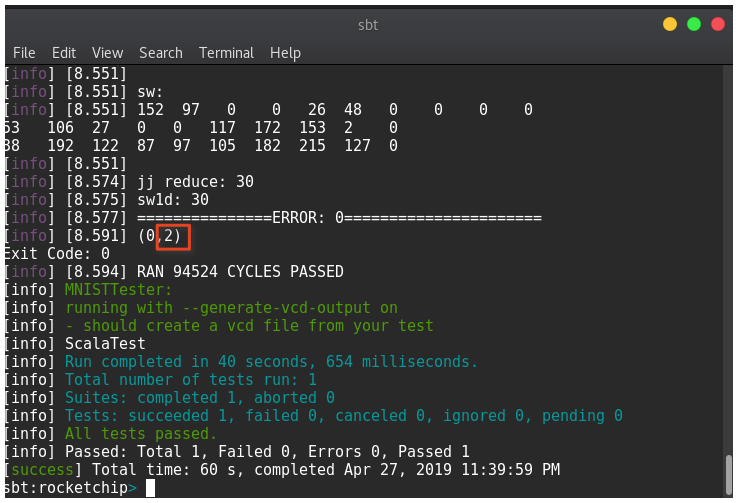
\includegraphics[scale=0.6]{../pdf/2_result.png}\\
    \caption{测试结果为2}
    \label{2_result}
\end{figure}
    输入一个32×32的矩阵,其代表了一个手写数字2,如图\ref{2}所示。
    经过图\ref{mnist_k}流程,最终\emph{argmax}函数输出结果为2,如图\ref{2_result}所示。
    测试过程中,加速器计算的每一个结果都有软件设计的仿真器与其进行比对,并记录错误数,最终从图\ref{2_result}可以看出输出的ERROR数为0。

    经过测试,本文设计的卷积计算加速器可以稳定、准确计算多卷积核、多通道、多图片的卷积计算,并且通过LeNet模型测试。

\section{系统性能}
    \subsection{资源占用}
    目前几乎所有的EDA工具都只是针对Verilog或VHDL进行开发,因此Chisel3开发的最后一步就是生成Verilog文件,供其他EDA工具使用。

    本文设计之初使用的RAM是Chisel3提供的MEM工具,虽然生成的Verilog文件也可综合,但其采用寄存器组堆叠的构造造成了资源极大的浪费。
    一个内部RAM采用MEM,深度为256,宽度为16bit的6×7PE阵列,其综合结果如图\ref{mem_res}。
    \begin{figure}[h]
        \centering
        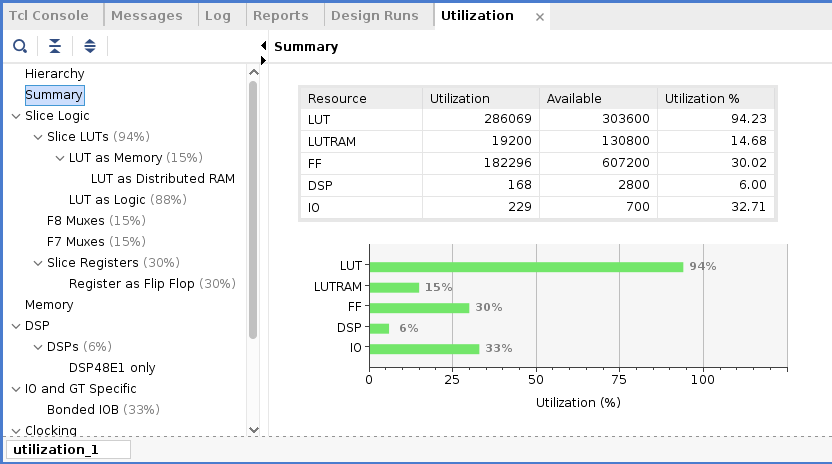
\includegraphics[scale=0.5]{../pdf/old_resource.png}\\
        \caption{使用MEM的资源报告}
        \label{mem_res}
    \end{figure}
    同等规格的RAM若采用本文第四章所述的优化方案之后,其资源占用率大大下降,综合结果如图\ref{dw_res}。
    \begin{figure}[h]
        \centering
        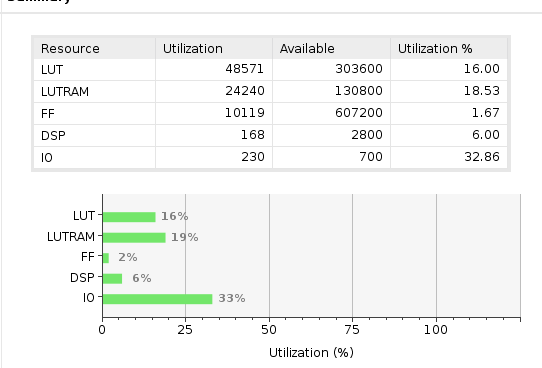
\includegraphics[scale=0.5]{../pdf/new_resource.png}\\
        \caption{使用DW ip的资源报告}
        \label{dw_res}
    \end{figure}

    \subsection{时序报告}
    采用Chisel3 MEM的6×7大小的PE阵列其时序报告如图\ref{mem_time}所示。
    \begin{figure}[h]
        \centering
        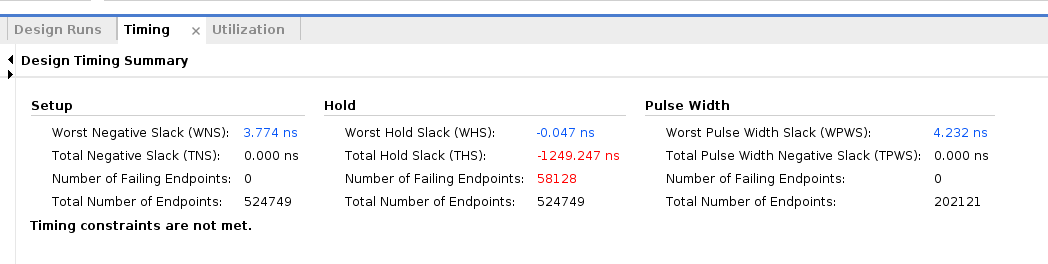
\includegraphics[scale=0.4]{../pdf/old_time.png}\\
        \caption{100M时钟下使用MEM的时序报告}
        \label{mem_time}
    \end{figure}
    使用Designware IP优化之后的时序报告如图\ref{dw_time}所示。
    \begin{figure}[h]
        \centering
        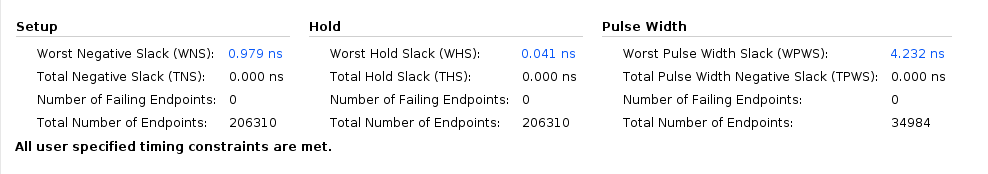
\includegraphics[scale=0.4]{../pdf/new_time.png}\\
        \caption{100M时钟下使用DW ip的时序报告}
        \label{dw_time}
    \end{figure}
    从时序报告中可以看出,采用了MEM方案的PE阵列在工作频率上有这将近20\%的优势,但却牺牲了将近5倍的资源。

\section{本章小结}
本章首先依次介绍了关键模块的仿真时序图,并根据时序图详细描述了模块的逻辑行为。之后,采用一量化的LeNet网络进行了手写数字识别测试,通过测试结果,证明了本文设计
的用于CNN加速的PE阵列生成器的能够生成指定规模的PE阵列,并能正确的按照行静止卷积法进行卷积计算。
% \subsection{二级节标题}

% \subsubsection{三级节标题}

% \paragraph{四级节标题}

% \subparagraph{五级节标题}

% \section{脚注}

% Lorem ipsum dolor sit amet, consectetur adipiscing elit, sed do eiusmod tempor
% incididunt ut labore et dolore magna aliqua. Ut enim ad minim veniam, quis
% nostrud exercitation ullamco laboris nisi ut aliquip ex ea commodo consequat.
% Duis aute irure dolor in reprehenderit in voluptate velit esse cillum dolore eu
% fugiat nulla pariatur. Excepteur sint occaecat cupidatat non proident, sunt in
% culpa qui officia deserunt mollit anim id est laborum.
% \footnote{This is a long long long long long long long long long long long long
% long long long long long long long long long long footnote.}
